% Options for packages loaded elsewhere
% Options for packages loaded elsewhere
\PassOptionsToPackage{unicode}{hyperref}
\PassOptionsToPackage{hyphens}{url}
%
\documentclass[
  english,
  russian,
  12pt,
  a4paper,
  DIV=11,
  numbers=noendperiod]{scrreprt}
\usepackage{xcolor}
\usepackage[margin=2cm]{geometry}
\usepackage{amsmath,amssymb}
\setcounter{secnumdepth}{5}
\usepackage{iftex}
\ifPDFTeX
  \usepackage[T1]{fontenc}
  \usepackage[utf8]{inputenc}
  \usepackage{textcomp} % provide euro and other symbols
\else % if luatex or xetex
  \usepackage{unicode-math} % this also loads fontspec
  \defaultfontfeatures{Scale=MatchLowercase}
  \defaultfontfeatures[\rmfamily]{Ligatures=TeX,Scale=1}
\fi
\usepackage{lmodern}
\ifPDFTeX\else
  % xetex/luatex font selection
  \setmainfont[]{DejaVu Sans}
  \setmonofont[]{DejaVu Sans Mono}
\fi
% Use upquote if available, for straight quotes in verbatim environments
\IfFileExists{upquote.sty}{\usepackage{upquote}}{}
\IfFileExists{microtype.sty}{% use microtype if available
  \usepackage[]{microtype}
  \UseMicrotypeSet[protrusion]{basicmath} % disable protrusion for tt fonts
}{}
\usepackage{setspace}
% Make \paragraph and \subparagraph free-standing
\makeatletter
\ifx\paragraph\undefined\else
  \let\oldparagraph\paragraph
  \renewcommand{\paragraph}{
    \@ifstar
      \xxxParagraphStar
      \xxxParagraphNoStar
  }
  \newcommand{\xxxParagraphStar}[1]{\oldparagraph*{#1}\mbox{}}
  \newcommand{\xxxParagraphNoStar}[1]{\oldparagraph{#1}\mbox{}}
\fi
\ifx\subparagraph\undefined\else
  \let\oldsubparagraph\subparagraph
  \renewcommand{\subparagraph}{
    \@ifstar
      \xxxSubParagraphStar
      \xxxSubParagraphNoStar
  }
  \newcommand{\xxxSubParagraphStar}[1]{\oldsubparagraph*{#1}\mbox{}}
  \newcommand{\xxxSubParagraphNoStar}[1]{\oldsubparagraph{#1}\mbox{}}
\fi
\makeatother

\usepackage{color}
\usepackage{fancyvrb}
\newcommand{\VerbBar}{|}
\newcommand{\VERB}{\Verb[commandchars=\\\{\}]}
\DefineVerbatimEnvironment{Highlighting}{Verbatim}{commandchars=\\\{\}}
% Add ',fontsize=\small' for more characters per line
\usepackage{framed}
\definecolor{shadecolor}{RGB}{241,243,245}
\newenvironment{Shaded}{\begin{snugshade}}{\end{snugshade}}
\newcommand{\AlertTok}[1]{\textcolor[rgb]{0.68,0.00,0.00}{#1}}
\newcommand{\AnnotationTok}[1]{\textcolor[rgb]{0.37,0.37,0.37}{#1}}
\newcommand{\AttributeTok}[1]{\textcolor[rgb]{0.40,0.45,0.13}{#1}}
\newcommand{\BaseNTok}[1]{\textcolor[rgb]{0.68,0.00,0.00}{#1}}
\newcommand{\BuiltInTok}[1]{\textcolor[rgb]{0.00,0.23,0.31}{#1}}
\newcommand{\CharTok}[1]{\textcolor[rgb]{0.13,0.47,0.30}{#1}}
\newcommand{\CommentTok}[1]{\textcolor[rgb]{0.37,0.37,0.37}{#1}}
\newcommand{\CommentVarTok}[1]{\textcolor[rgb]{0.37,0.37,0.37}{\textit{#1}}}
\newcommand{\ConstantTok}[1]{\textcolor[rgb]{0.56,0.35,0.01}{#1}}
\newcommand{\ControlFlowTok}[1]{\textcolor[rgb]{0.00,0.23,0.31}{\textbf{#1}}}
\newcommand{\DataTypeTok}[1]{\textcolor[rgb]{0.68,0.00,0.00}{#1}}
\newcommand{\DecValTok}[1]{\textcolor[rgb]{0.68,0.00,0.00}{#1}}
\newcommand{\DocumentationTok}[1]{\textcolor[rgb]{0.37,0.37,0.37}{\textit{#1}}}
\newcommand{\ErrorTok}[1]{\textcolor[rgb]{0.68,0.00,0.00}{#1}}
\newcommand{\ExtensionTok}[1]{\textcolor[rgb]{0.00,0.23,0.31}{#1}}
\newcommand{\FloatTok}[1]{\textcolor[rgb]{0.68,0.00,0.00}{#1}}
\newcommand{\FunctionTok}[1]{\textcolor[rgb]{0.28,0.35,0.67}{#1}}
\newcommand{\ImportTok}[1]{\textcolor[rgb]{0.00,0.46,0.62}{#1}}
\newcommand{\InformationTok}[1]{\textcolor[rgb]{0.37,0.37,0.37}{#1}}
\newcommand{\KeywordTok}[1]{\textcolor[rgb]{0.00,0.23,0.31}{\textbf{#1}}}
\newcommand{\NormalTok}[1]{\textcolor[rgb]{0.00,0.23,0.31}{#1}}
\newcommand{\OperatorTok}[1]{\textcolor[rgb]{0.37,0.37,0.37}{#1}}
\newcommand{\OtherTok}[1]{\textcolor[rgb]{0.00,0.23,0.31}{#1}}
\newcommand{\PreprocessorTok}[1]{\textcolor[rgb]{0.68,0.00,0.00}{#1}}
\newcommand{\RegionMarkerTok}[1]{\textcolor[rgb]{0.00,0.23,0.31}{#1}}
\newcommand{\SpecialCharTok}[1]{\textcolor[rgb]{0.37,0.37,0.37}{#1}}
\newcommand{\SpecialStringTok}[1]{\textcolor[rgb]{0.13,0.47,0.30}{#1}}
\newcommand{\StringTok}[1]{\textcolor[rgb]{0.13,0.47,0.30}{#1}}
\newcommand{\VariableTok}[1]{\textcolor[rgb]{0.07,0.07,0.07}{#1}}
\newcommand{\VerbatimStringTok}[1]{\textcolor[rgb]{0.13,0.47,0.30}{#1}}
\newcommand{\WarningTok}[1]{\textcolor[rgb]{0.37,0.37,0.37}{\textit{#1}}}

\usepackage{longtable,booktabs,array}
\newcounter{none} % for unnumbered tables
\usepackage{calc} % for calculating minipage widths
% Correct order of tables after \paragraph or \subparagraph
\usepackage{etoolbox}
\makeatletter
\patchcmd\longtable{\par}{\if@noskipsec\mbox{}\fi\par}{}{}
\makeatother
% Allow footnotes in longtable head/foot
\IfFileExists{footnotehyper.sty}{\usepackage{footnotehyper}}{\usepackage{footnote}}
\makesavenoteenv{longtable}
\usepackage{graphicx}
\makeatletter
\newsavebox\pandoc@box
\newcommand*\pandocbounded[1]{% scales image to fit in text height/width
  \sbox\pandoc@box{#1}%
  \Gscale@div\@tempa{\textheight}{\dimexpr\ht\pandoc@box+\dp\pandoc@box\relax}%
  \Gscale@div\@tempb{\linewidth}{\wd\pandoc@box}%
  \ifdim\@tempb\p@<\@tempa\p@\let\@tempa\@tempb\fi% select the smaller of both
  \ifdim\@tempa\p@<\p@\scalebox{\@tempa}{\usebox\pandoc@box}%
  \else\usebox{\pandoc@box}%
  \fi%
}
% Set default figure placement to htbp
\def\fps@figure{htbp}
\makeatother



\ifLuaTeX
\usepackage[bidi=basic,shorthands=off,provide=*]{babel}
\else
\usepackage[bidi=default,shorthands=off,provide=*]{babel}
\fi
\ifPDFTeX
\else
\babelfont{rm}[]{DejaVu Sans}
\fi
\ifLuaTeX
  \usepackage{selnolig} % disable illegal ligatures
\fi


\setlength{\emergencystretch}{3em} % prevent overfull lines

\providecommand{\tightlist}{%
  \setlength{\itemsep}{0pt}\setlength{\parskip}{0pt}}



 
\usepackage[style=gost-numeric,backend=biber,langhook=extras,autolang=other*]{biblatex}
\addbibresource{bib/cite.bib}

\usepackage[]{csquotes}

\usepackage{indentfirst}
\usepackage{float}
\floatplacement{figure}{H}
\IfFileExists{plex-otf.sty}{
  %% Full TeXlive
  \usepackage[
    % math,
    RM={Scale=0.94},SS={Scale=0.94},SScon={Scale=0.94},TT={Scale=MatchLowercase,FakeStretch=0.9},
    DefaultFeatures={Ligatures=Common}
  ]{plex-otf}
  % \usepackage[Scale=MatchUppercase]{juliamono}
}{
  %% TinyTeX
  \usepackage{libertine}
}
\KOMAoption{captions}{tableheading}
\makeatletter
\@ifpackageloaded{caption}{}{\usepackage{caption}}
\AtBeginDocument{%
\ifdefined\contentsname
  \renewcommand*\contentsname{Содержание}
\else
  \newcommand\contentsname{Содержание}
\fi
\ifdefined\listfigurename
  \renewcommand*\listfigurename{Список иллюстраций}
\else
  \newcommand\listfigurename{Список иллюстраций}
\fi
\ifdefined\listtablename
  \renewcommand*\listtablename{Список таблиц}
\else
  \newcommand\listtablename{Список таблиц}
\fi
\ifdefined\figurename
  \renewcommand*\figurename{Рисунок}
\else
  \newcommand\figurename{Рисунок}
\fi
\ifdefined\tablename
  \renewcommand*\tablename{Таблица}
\else
  \newcommand\tablename{Таблица}
\fi
}
\@ifpackageloaded{float}{}{\usepackage{float}}
\floatstyle{ruled}
\@ifundefined{c@chapter}{\newfloat{codelisting}{h}{lop}}{\newfloat{codelisting}{h}{lop}[chapter]}
\floatname{codelisting}{Список}
\newcommand*\listoflistings{\listof{codelisting}{Листинги}}
\makeatother
\makeatletter
\makeatother
\makeatletter
\@ifpackageloaded{caption}{}{\usepackage{caption}}
\@ifpackageloaded{subcaption}{}{\usepackage{subcaption}}
\makeatother
\usepackage{bookmark}
\IfFileExists{xurl.sty}{\usepackage{xurl}}{} % add URL line breaks if available
\urlstyle{same}
% fallback for those not using the hyperref driver hyperxmp:
\makeatletter
\@ifundefined{xmpquote}{\newcommand{\xmpquote}[1]{#1}}{}
\makeatother
\hypersetup{
  pdftitle={Лабораторная работа № 5},
  pdfauthor={Нечаева Кира Андреевна},
  pdflang={ru-RU},
  hidelinks,
  pdfcreator={LaTeX via pandoc}}


\title{Лабораторная работа № 5}
\usepackage{etoolbox}
\makeatletter
\providecommand{\subtitle}[1]{% add subtitle to \maketitle
  \apptocmd{\@title}{\par {\large #1 \par}}{}{}
}
\makeatother
\subtitle{Моделирование с использованием сетей Петри}
\author{Нечаева Кира Андреевна}
\date{2026-01-01}
\begin{document}
\maketitle

\renewcommand*\contentsname{Содержание}
{
\setcounter{tocdepth}{1}
\tableofcontents
}
\listoffigures
\listoftables

\setstretch{1.5}
\chapter{Цель
работы}\label{ux446ux435ux43bux44c-ux440ux430ux431ux43eux442ux44b}

Цель лабораторной работы --- изучить применение сетей Петри для
моделирования дискретных систем на примере задачи «Обедающие философы».

В работе реализованы классическая сеть Петри и модифицированная сеть с
арбитром. Для них проведены стохастическое и детерминированное
моделирование, выполнена программная проверка возникновения взаимной
блокировки, создана анимация и проведено параметрическое исследование.

\chapter{Подготовка рабочего
окружения}\label{ux43fux43eux434ux433ux43eux442ux43eux432ux43aux430-ux440ux430ux431ux43eux447ux435ux433ux43e-ux43eux43aux440ux443ux436ux435ux43dux438ux44f}

Работа выполнялась в Ubuntu через WSL. Проект размещён в общем
репозитории лабораторных работ и ведётся в ветке \texttt{develop}.

\begin{figure}[H]

{\centering 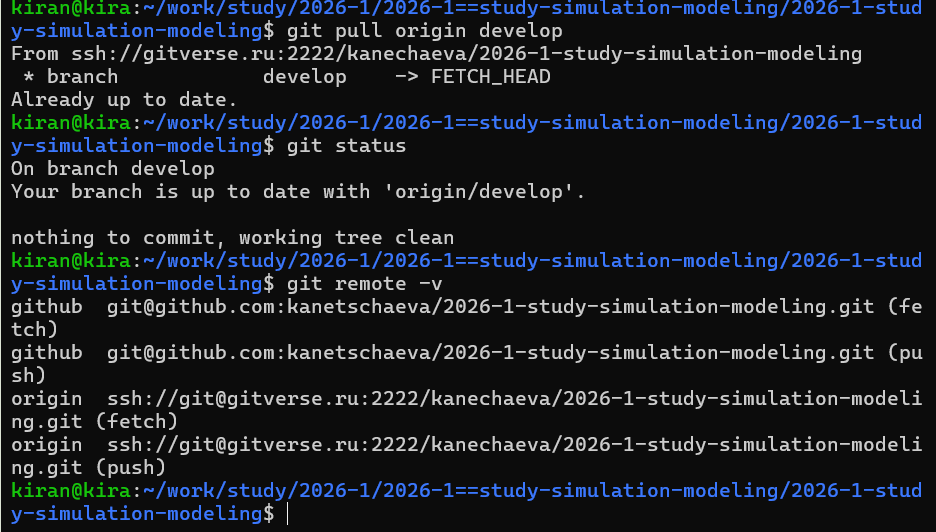
\includegraphics[width=0.95\linewidth,height=\textheight,keepaspectratio]{image/1.png}

}

\caption{Проверка репозитория и рабочей ветки}

\end{figure}%

Для лабораторной работы было создано отдельное окружение Julia и
установлены библиотеки для численного моделирования, обработки данных,
визуализации, литературного программирования и работы с Jupyter
Notebook.

\begin{figure}[H]

{\centering 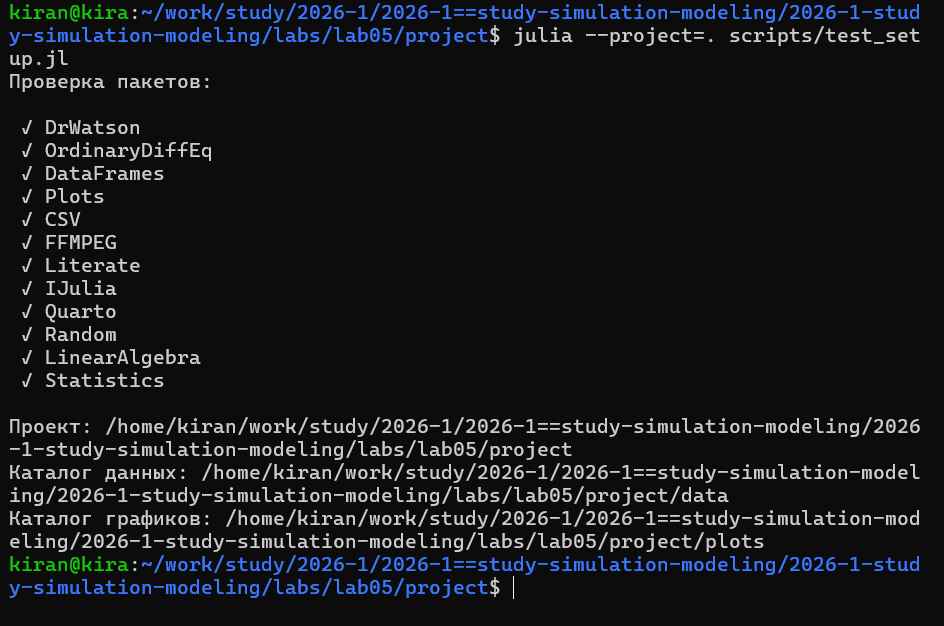
\includegraphics[width=0.95\linewidth,height=\textheight,keepaspectratio]{image/2.png}

}

\caption{Проверка используемых пакетов}

\end{figure}%

\chapter{Реализация сети
Петри}\label{ux440ux435ux430ux43bux438ux437ux430ux446ux438ux44f-ux441ux435ux442ux438-ux43fux435ux442ux440ux438}

Для представления сети была реализована структура \texttt{PetriNet},
которая хранит количество позиций, переходов, матрицу инцидентности и
имена элементов.

Для пяти философов классическая сеть содержит 20 позиций и 15 переходов.

В модели с арбитром появляется дополнительная позиция. В ней изначально
находится \texttt{N\ -\ 1} фишек, поэтому все философы не могут
одновременно начать захват ресурсов.

Перед основными экспериментами была проведена отдельная проверка
построения обеих сетей и короткий тест стохастического моделирования.

\begin{figure}[H]

{\centering 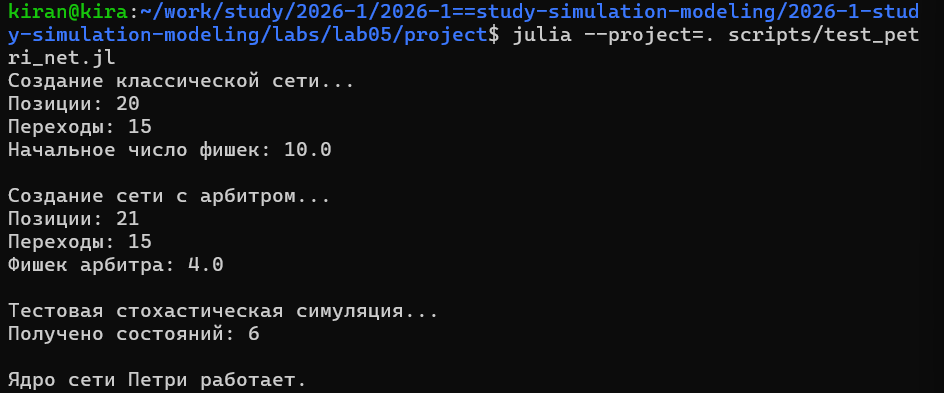
\includegraphics[width=0.95\linewidth,height=\textheight,keepaspectratio]{image/3.png}

}

\caption{Проверка ядра сети Петри}

\end{figure}%

\chapter{Стохастическое
моделирование}\label{ux441ux442ux43eux445ux430ux441ux442ux438ux447ux435ux441ux43aux43eux435-ux43cux43eux434ux435ux43bux438ux440ux43eux432ux430ux43dux438ux435}

Для стохастической модели использован алгоритм Гиллеспи.

Состояние сети меняется отдельными срабатываниями переходов. Выбор
следующего перехода и времени его срабатывания зависит от текущего
состояния сети.

Классическая сеть и сеть с арбитром запускались с одинаковым значением
\texttt{seed}. Это позволяет сравнивать модели при одинаковой
последовательности псевдослучайных чисел.

После симуляции программа автоматически проверяет доступность переходов.
Если ни один переход больше не может сработать, фиксируется
\texttt{deadlock}.

\begin{figure}[H]

{\centering 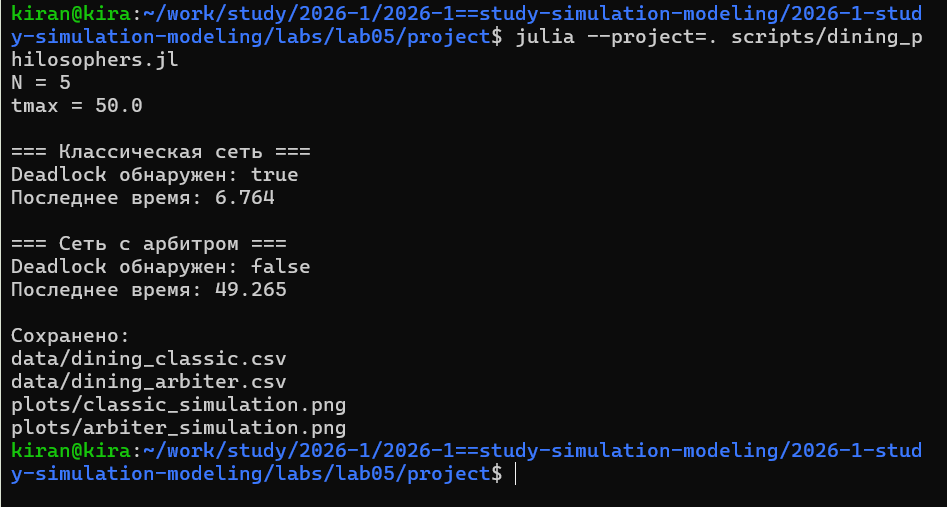
\includegraphics[width=0.95\linewidth,height=\textheight,keepaspectratio]{image/4.png}

}

\caption{Результат стохастического эксперимента}

\end{figure}%

\begin{figure}[H]

{\centering 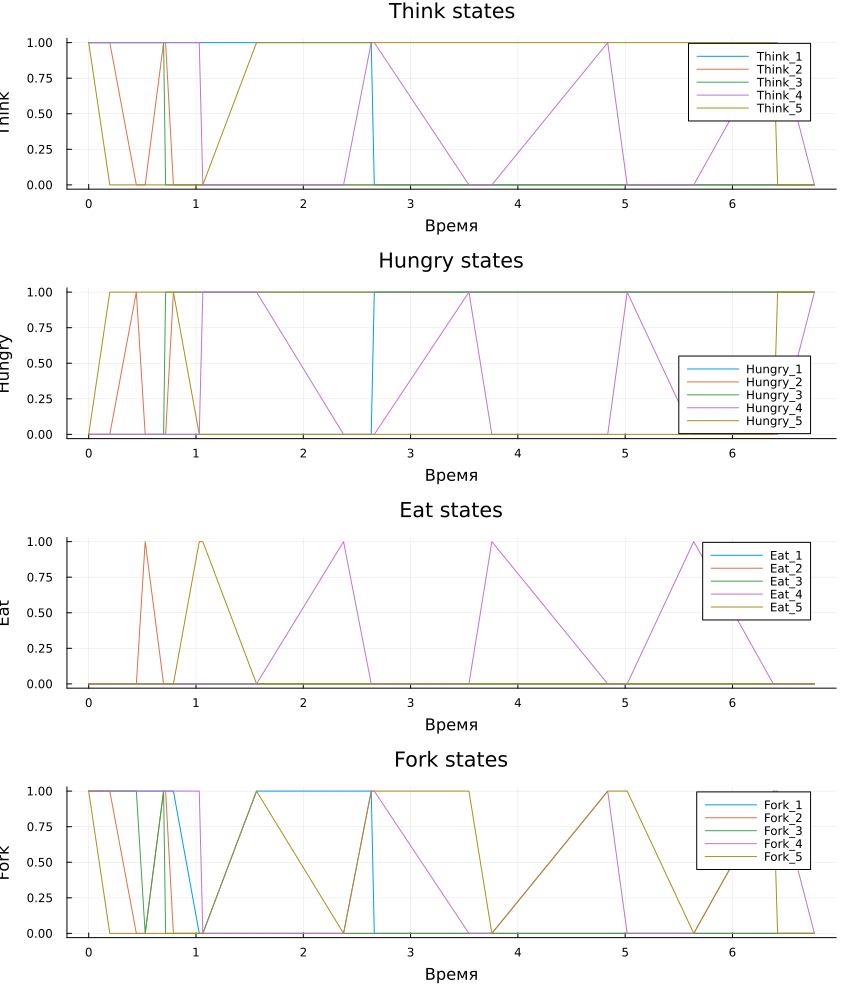
\includegraphics[width=0.9\linewidth,height=\textheight,keepaspectratio]{image/plots/classic_simulation.png}

}

\caption{Стохастическая динамика классической сети}

\end{figure}%

\begin{figure}[H]

{\centering 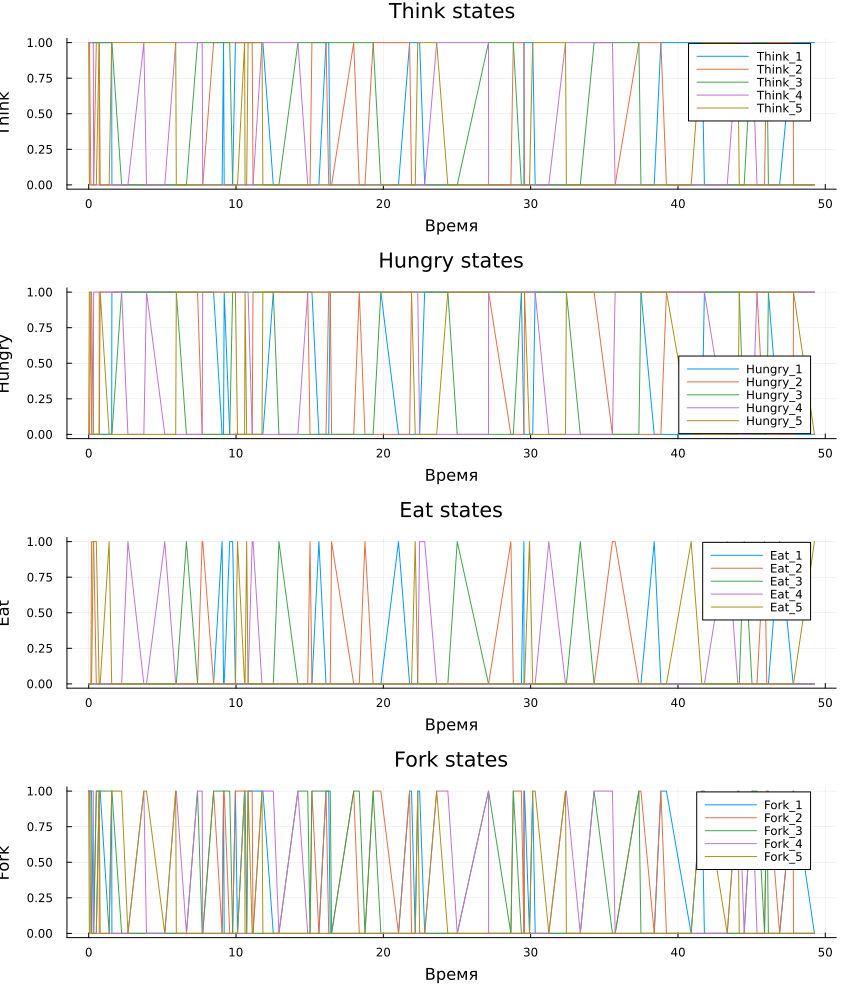
\includegraphics[width=0.9\linewidth,height=\textheight,keepaspectratio]{image/plots/arbiter_simulation.png}

}

\caption{Стохастическая динамика сети с арбитром}

\end{figure}%

\chapter{Детерминированное
моделирование}\label{ux434ux435ux442ux435ux440ux43cux438ux43dux438ux440ux43eux432ux430ux43dux43dux43eux435-ux43cux43eux434ux435ux43bux438ux440ux43eux432ux430ux43dux438ux435}

Дополнительно была исследована детерминированная версия модели.

Матрица инцидентности сети используется для формирования системы
дифференциальных уравнений. Поэтому здесь получается непрерывная
траектория изменения состояний вместо последовательности отдельных
случайных событий.

\begin{figure}[H]

{\centering 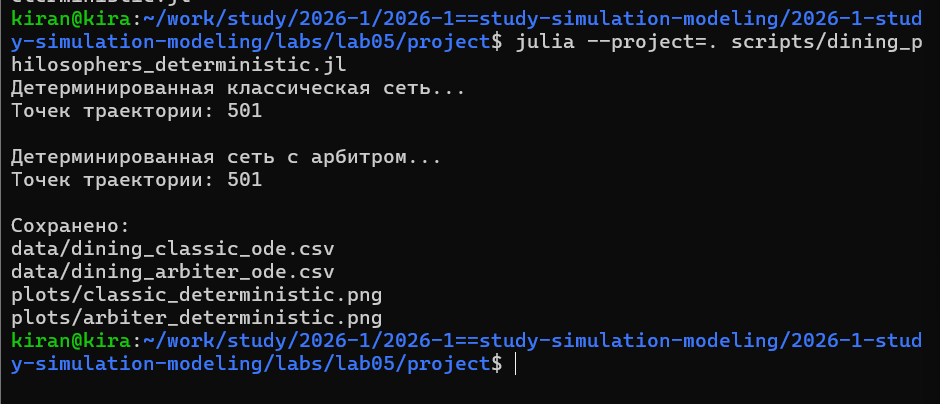
\includegraphics[width=0.95\linewidth,height=\textheight,keepaspectratio]{image/5.png}

}

\caption{Выполнение детерминированного моделирования}

\end{figure}%

\begin{figure}[H]

{\centering 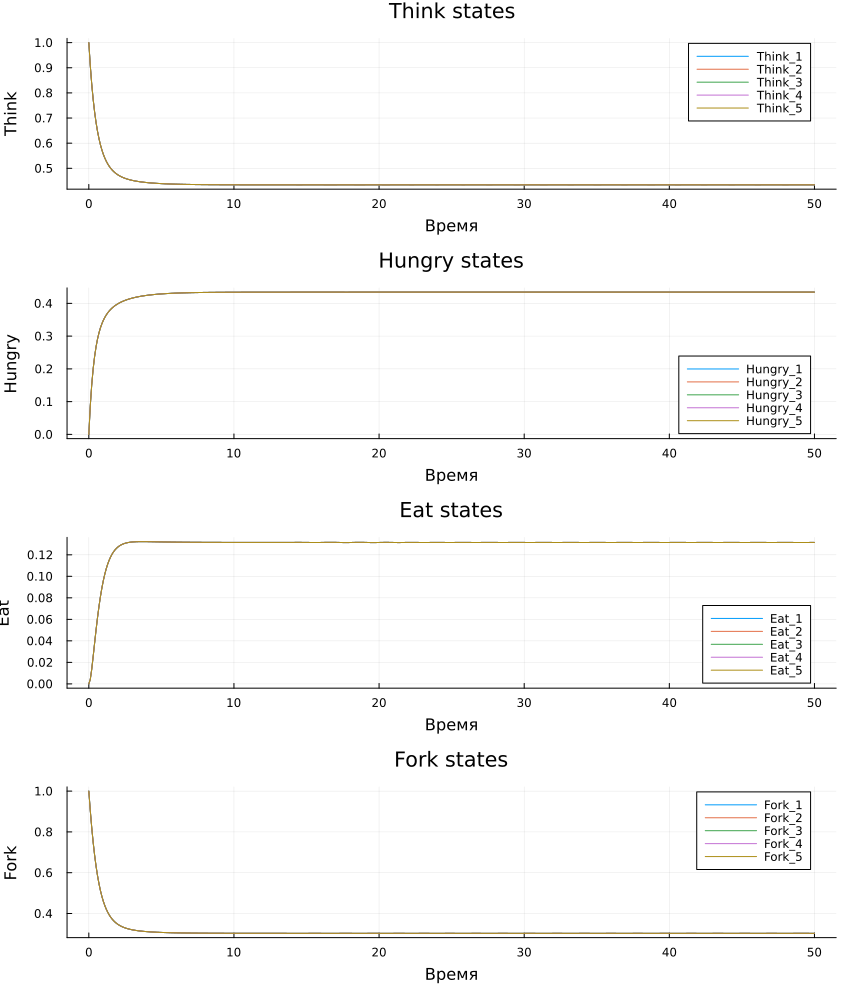
\includegraphics[width=0.9\linewidth,height=\textheight,keepaspectratio]{image/plots/classic_deterministic.png}

}

\caption{Детерминированная динамика классической сети}

\end{figure}%

\begin{figure}[H]

{\centering 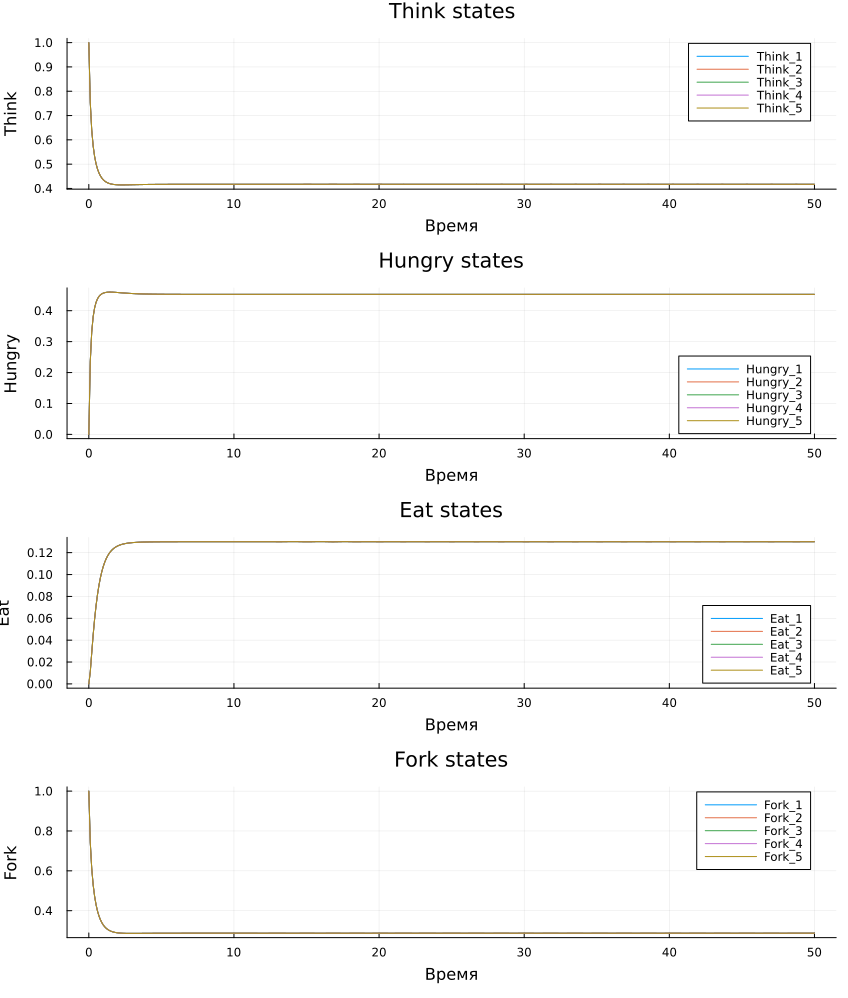
\includegraphics[width=0.9\linewidth,height=\textheight,keepaspectratio]{image/plots/arbiter_deterministic.png}

}

\caption{Детерминированная динамика сети с арбитром}

\end{figure}%

\chapter{Анимация работы
сети}\label{ux430ux43dux438ux43cux430ux446ux438ux44f-ux440ux430ux431ux43eux442ux44b-ux441ux435ux442ux438}

Для дополнительной визуализации была создана GIF-анимация.

В анимации использованы три философа. Такое уменьшение количества
участников позволяет лучше видеть отдельные позиции и изменение
количества фишек.

\begin{figure}[H]

{\centering 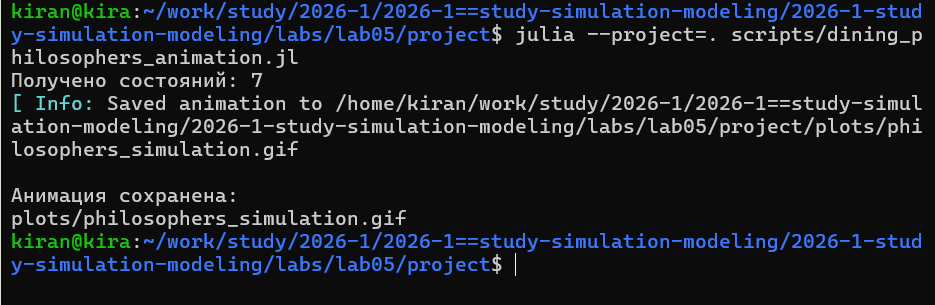
\includegraphics[width=0.95\linewidth,height=\textheight,keepaspectratio]{image/6.png}

}

\caption{Создание GIF-анимации}

\end{figure}%

Анимация сохранена в файле:

\texttt{image/plots/philosophers\_simulation.gif}.

\chapter{Итоговое
сравнение}\label{ux438ux442ux43eux433ux43eux432ux43eux435-ux441ux440ux430ux432ux43dux435ux43dux438ux435}

Для итогового сравнения используются ранее сохранённые результаты
моделирования.

Скрипт загружает CSV-файлы и анализирует состояния \texttt{Eat\_i} для
всех философов. Повторная симуляция при этом не выполняется.

\begin{figure}[H]

{\centering 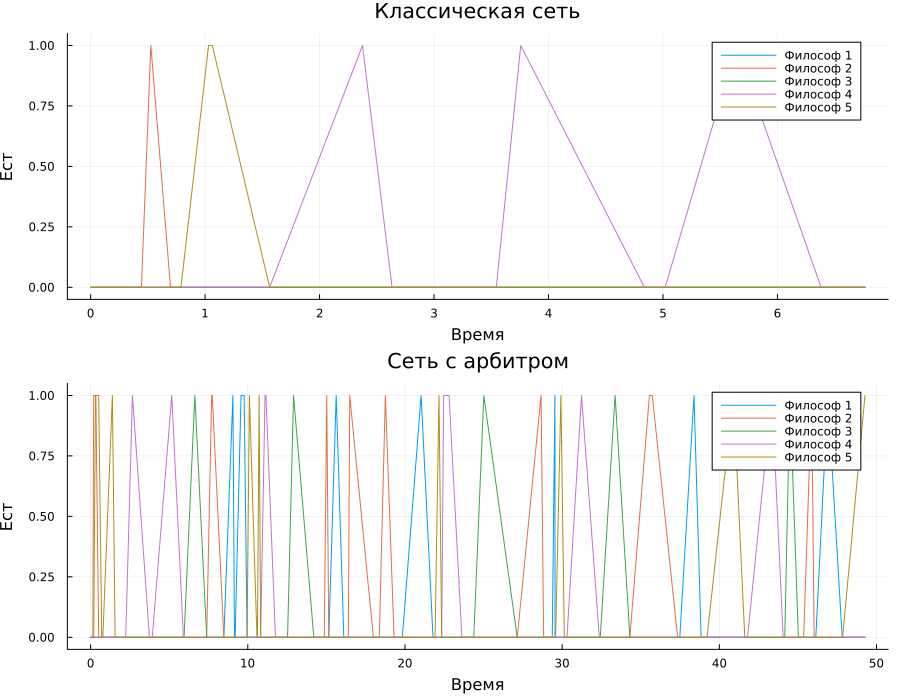
\includegraphics[width=0.9\linewidth,height=\textheight,keepaspectratio]{image/plots/final_report.png}

}

\caption{Сравнение состояний Eat в двух моделях}

\end{figure}%

В классической модели длительное отсутствие философов в состоянии
\texttt{Eat} соответствует взаимной блокировке. В сети с арбитром доступ
к ресурсам сохраняется.

\chapter{Параметрическое
исследование}\label{ux43fux430ux440ux430ux43cux435ux442ux440ux438ux447ux435ux441ux43aux43eux435-ux438ux441ux441ux43bux435ux434ux43eux432ux430ux43dux438ux435}

Стохастическая модель может давать разные траектории при разных
последовательностях случайных чисел.

Поэтому дополнительное исследование проводилось для нескольких
параметров:

\begin{itemize}
\tightlist
\item
  \texttt{N\ =\ 3};
\item
  \texttt{N\ =\ 5};
\item
  \texttt{N\ =\ 7};
\item
  нескольких значений \texttt{seed}.
\end{itemize}

Для каждой комбинации параметров отдельно моделировалась классическая
сеть и сеть с арбитром.

После этого программа рассчитывала долю запусков, завершившихся взаимной
блокировкой.

\begin{figure}[H]

{\centering 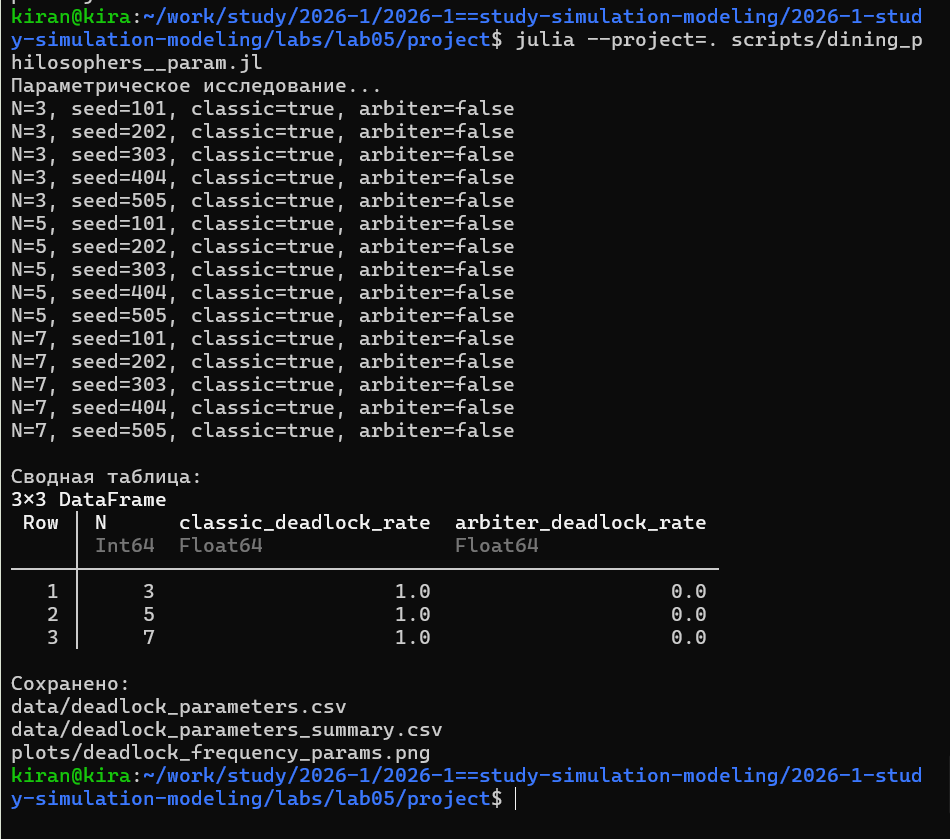
\includegraphics[width=0.95\linewidth,height=\textheight,keepaspectratio]{image/8.png}

}

\caption{Параметрическое исследование}

\end{figure}%

\begin{figure}[H]

{\centering 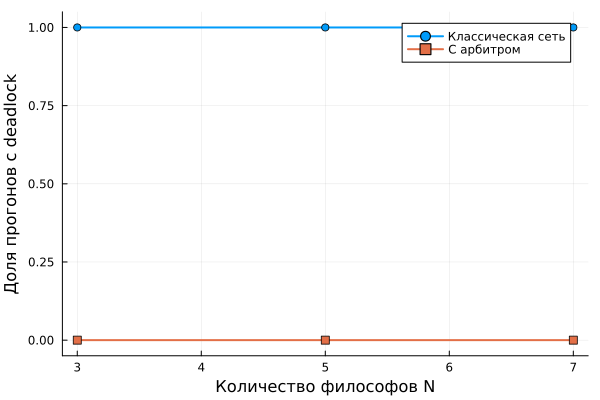
\includegraphics[width=0.9\linewidth,height=\textheight,keepaspectratio]{image/plots/deadlock_frequency_params.png}

}

\caption{Частота возникновения deadlock}

\end{figure}%

Использование нескольких повторных запусков позволяет оценивать не
отдельную случайную траекторию, а устойчивость результата.

\chapter{Литературное
программирование}\label{ux43bux438ux442ux435ux440ux430ux442ux443ux440ux43dux43eux435-ux43fux440ux43eux433ux440ux430ux43cux43cux438ux440ux43eux432ux430ux43dux438ux435}

Основные вычислительные сценарии были оформлены в литературном стиле.

Из одного исходного файла автоматически создаются:

\begin{itemize}
\tightlist
\item
  чистый Julia-код;
\item
  Jupyter Notebook;
\item
  документация Quarto.
\end{itemize}

Это позволяет поддерживать код и пояснение в одном исходнике.

\begin{figure}[H]

{\centering 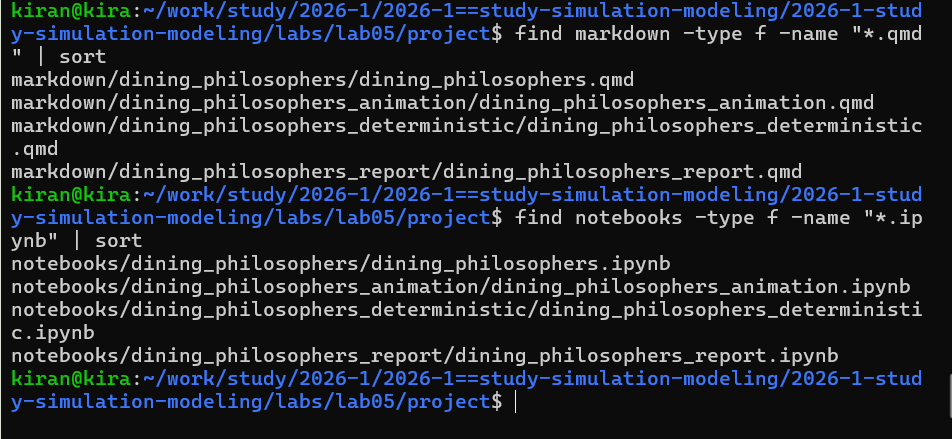
\includegraphics[width=0.95\linewidth,height=\textheight,keepaspectratio]{image/9.png}

}

\caption{Сгенерированные Quarto-документы и Jupyter Notebook}

\end{figure}%

\chapter{Проверка
воспроизводимости}\label{ux43fux440ux43eux432ux435ux440ux43aux430-ux432ux43eux441ux43fux440ux43eux438ux437ux432ux43eux434ux438ux43cux43eux441ux442ux438}

Автоматически созданные Jupyter Notebook были отдельно выполнены.

Это проверяет, что сгенерированные notebooks содержат все необходимые
команды и могут самостоятельно воспроизвести вычислительные
эксперименты.

\begin{figure}[H]

{\centering 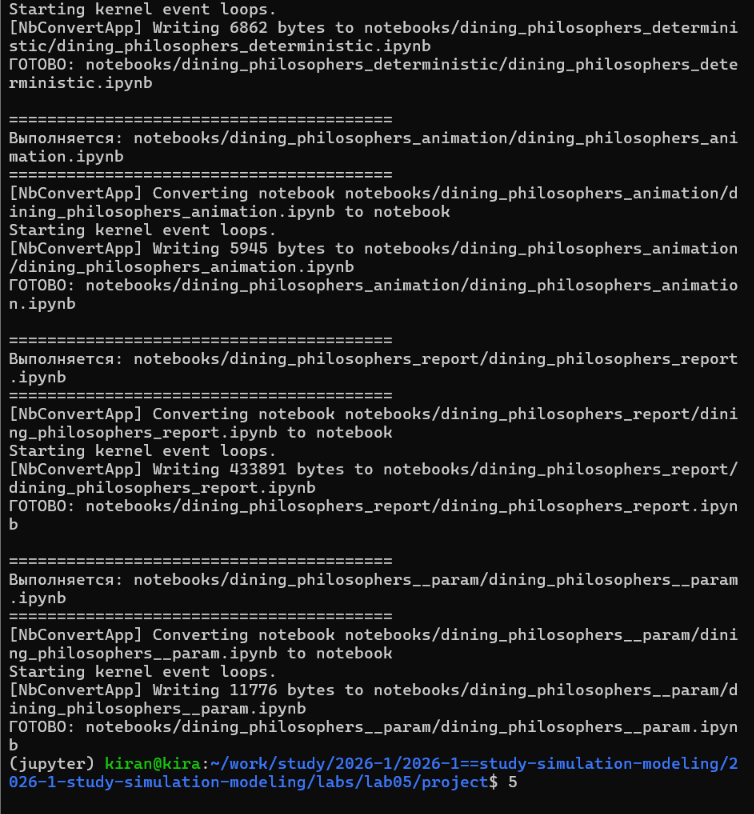
\includegraphics[width=0.95\linewidth,height=\textheight,keepaspectratio]{image/10.png}

}

\caption{Успешное выполнение Jupyter Notebook}

\end{figure}%

\chapter{Структура
проекта}\label{ux441ux442ux440ux443ux43aux442ux443ux440ux430-ux43fux440ux43eux435ux43aux442ux430}

После выполнения работы проект содержит исходный модуль сети Петри,
литературные программы, сгенерированные версии программ, notebooks,
документацию, таблицы, графики и анимацию.

\begin{figure}[H]

{\centering 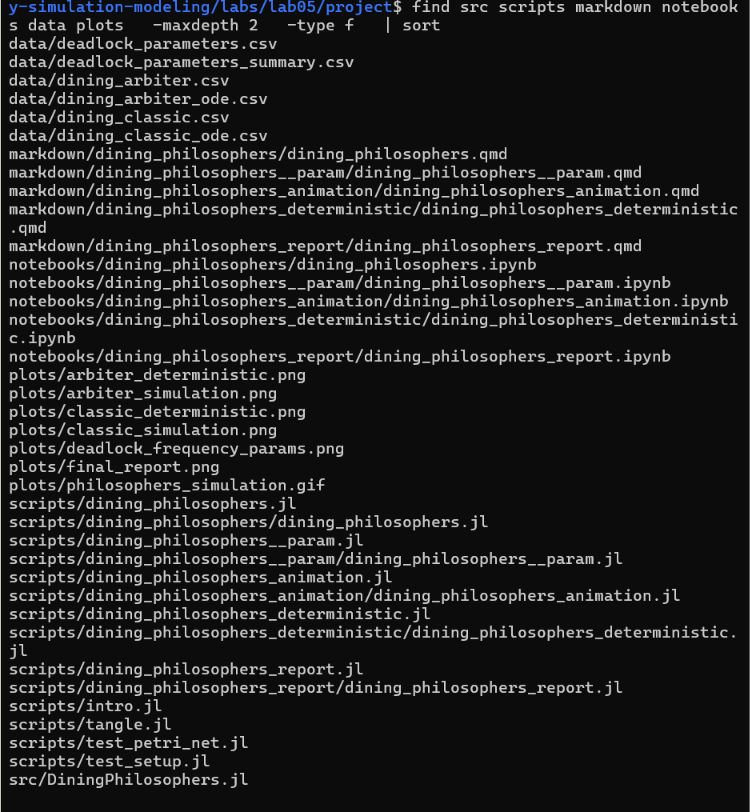
\includegraphics[width=0.95\linewidth,height=\textheight,keepaspectratio]{image/11.png}

}

\caption{Итоговая структура проекта}

\end{figure}%

\chapter{Контроль
версий}\label{ux43aux43eux43dux442ux440ux43eux43bux44c-ux432ux435ux440ux441ux438ux439}

Все изменения были сохранены в Git и отправлены в удалённые репозитории.

\begin{figure}[H]

{\centering 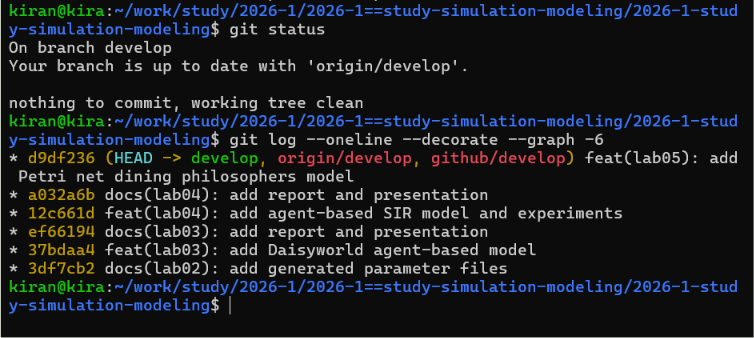
\includegraphics[width=0.95\linewidth,height=\textheight,keepaspectratio]{image/12.png}

}

\caption{Финальное состояние Git}

\end{figure}%

\chapter{Выводы}\label{ux432ux44bux432ux43eux434ux44b}

В лабораторной работе была реализована задача «Обедающие философы» с
использованием аппарата сетей Петри.

Были построены классическая сеть и сеть с дополнительным арбитром. Для
обеих моделей выполнено стохастическое и детерминированное
моделирование.

Программная проверка состояния сети позволяет автоматически обнаруживать
взаимную блокировку. Добавление арбитра изменяет правило распределения
ресурсов и предотвращает ситуацию, когда все философы одновременно
удерживают только одну вилку и ожидают вторую.

Дополнительно было проведено параметрическое исследование для различного
числа философов и нескольких случайных траекторий.

Все основные вычисления оформлены в литературном стиле, а автоматически
созданные Jupyter Notebook отдельно выполнены для проверки
воспроизводимости.

\chapter*{Приложение А. Quarto-документация основного
эксперимента}\label{ux43fux440ux438ux43bux43eux436ux435ux43dux438ux435-ux430.-quarto-ux434ux43eux43aux443ux43cux435ux43dux442ux430ux446ux438ux44f-ux43eux441ux43dux43eux432ux43dux43eux433ux43e-ux44dux43aux441ux43fux435ux440ux438ux43cux435ux43dux442ux430}
\addcontentsline{toc}{chapter}{Приложение А. Quarto-документация
основного эксперимента}

Ниже интегрирована статическая версия документации Quarto, автоматически
созданной из литературного исходного кода.

\chapter{Обедающие философы: стохастическая
модель}\label{ux43eux431ux435ux434ux430ux44eux449ux438ux435-ux444ux438ux43bux43eux441ux43eux444ux44b-ux441ux442ux43eux445ux430ux441ux442ux438ux447ux435ux441ux43aux430ux44f-ux43cux43eux434ux435ux43bux44c}

\textbf{Автор:} Нечаева Кира Андреевна

\textbf{Группа:} НКНбд-01-23

Сравниваются классическая сеть Петри и сеть с дополнительным арбитром.

\begin{Shaded}
\begin{Highlighting}[]
\ConstantTok{ENV}\NormalTok{[}\StringTok{"GKSwstype"}\NormalTok{] }\OperatorTok{=} \StringTok{"100"}

\ImportTok{using} \BuiltInTok{DrWatson}
\PreprocessorTok{@quickactivate} \StringTok{"project"}

\FunctionTok{include}\NormalTok{(}
    \FunctionTok{srcdir}\NormalTok{(}
        \StringTok{"DiningPhilosophers.jl"}
\NormalTok{    )}
\NormalTok{)}

\ImportTok{using} \BuiltInTok{.DiningPhilosophers}

\ImportTok{using} \BuiltInTok{DataFrames}
\ImportTok{using} \BuiltInTok{CSV}
\ImportTok{using} \BuiltInTok{Plots}
\ImportTok{using} \BuiltInTok{Random}
\end{Highlighting}
\end{Shaded}

\section{Параметры}\label{ux43fux430ux440ux430ux43cux435ux442ux440ux44b}

\begin{Shaded}
\begin{Highlighting}[]
\NormalTok{N }\OperatorTok{=}
    \FloatTok{5}

\NormalTok{tmax }\OperatorTok{=}
    \FloatTok{50.0}

\NormalTok{seed }\OperatorTok{=}
    \FloatTok{123}

\FunctionTok{println}\NormalTok{(}
    \StringTok{"N = "}\NormalTok{,}
\NormalTok{    N}
\NormalTok{)}

\FunctionTok{println}\NormalTok{(}
    \StringTok{"tmax = "}\NormalTok{,}
\NormalTok{    tmax}
\NormalTok{)}
\end{Highlighting}
\end{Shaded}

\section{Классическая
сеть}\label{ux43aux43bux430ux441ux441ux438ux447ux435ux441ux43aux430ux44f-ux441ux435ux442ux44c}

\begin{Shaded}
\begin{Highlighting}[]
\FunctionTok{println}\NormalTok{(}
    \StringTok{"}\SpecialCharTok{\textbackslash{}n}\StringTok{=== Классическая сеть ==="}
\NormalTok{)}

\NormalTok{net\_classic,}
\NormalTok{u0\_classic,}
\NormalTok{\_ }\OperatorTok{=}
    \FunctionTok{build\_classical\_network}\NormalTok{(}
\NormalTok{        N}
\NormalTok{    )}

\NormalTok{df\_classic }\OperatorTok{=}
    \FunctionTok{simulate\_stochastic}\NormalTok{(}
\NormalTok{        net\_classic,}
\NormalTok{        u0\_classic,}
\NormalTok{        tmax;}
\NormalTok{        rng}\OperatorTok{=}\FunctionTok{MersenneTwister}\NormalTok{(}
\NormalTok{            seed}
\NormalTok{        )}
\NormalTok{    )}

\NormalTok{CSV.}\FunctionTok{write}\NormalTok{(}
    \FunctionTok{datadir}\NormalTok{(}
        \StringTok{"dining\_classic.csv"}
\NormalTok{    ),}
\NormalTok{    df\_classic}
\NormalTok{)}

\NormalTok{dead\_classic }\OperatorTok{=}
    \FunctionTok{detect\_deadlock}\NormalTok{(}
\NormalTok{        df\_classic,}
\NormalTok{        net\_classic}
\NormalTok{    )}

\FunctionTok{println}\NormalTok{(}
    \StringTok{"Deadlock обнаружен: "}\NormalTok{,}
\NormalTok{    dead\_classic}
\NormalTok{)}

\FunctionTok{println}\NormalTok{(}
    \StringTok{"Последнее время: "}\NormalTok{,}
    \FunctionTok{round}\NormalTok{(}
\NormalTok{        df\_classic.time[}\KeywordTok{end}\NormalTok{],}
\NormalTok{        digits}\OperatorTok{=}\FloatTok{3}
\NormalTok{    )}
\NormalTok{)}

\NormalTok{plot\_classic }\OperatorTok{=}
    \FunctionTok{plot\_marking\_evolution}\NormalTok{(}
\NormalTok{        df\_classic,}
\NormalTok{        N}
\NormalTok{    )}

\FunctionTok{savefig}\NormalTok{(}
\NormalTok{    plot\_classic,}
    \FunctionTok{plotsdir}\NormalTok{(}
        \StringTok{"classic\_simulation.png"}
\NormalTok{    )}
\NormalTok{)}
\end{Highlighting}
\end{Shaded}

\section{Сеть с
арбитром}\label{ux441ux435ux442ux44c-ux441-ux430ux440ux431ux438ux442ux440ux43eux43c}

\begin{Shaded}
\begin{Highlighting}[]
\FunctionTok{println}\NormalTok{(}
    \StringTok{"}\SpecialCharTok{\textbackslash{}n}\StringTok{=== Сеть с арбитром ==="}
\NormalTok{)}

\NormalTok{net\_arbiter,}
\NormalTok{u0\_arbiter,}
\NormalTok{\_ }\OperatorTok{=}
    \FunctionTok{build\_arbiter\_network}\NormalTok{(}
\NormalTok{        N}
\NormalTok{    )}

\NormalTok{df\_arbiter }\OperatorTok{=}
    \FunctionTok{simulate\_stochastic}\NormalTok{(}
\NormalTok{        net\_arbiter,}
\NormalTok{        u0\_arbiter,}
\NormalTok{        tmax;}
\NormalTok{        rng}\OperatorTok{=}\FunctionTok{MersenneTwister}\NormalTok{(}
\NormalTok{            seed}
\NormalTok{        )}
\NormalTok{    )}

\NormalTok{CSV.}\FunctionTok{write}\NormalTok{(}
    \FunctionTok{datadir}\NormalTok{(}
        \StringTok{"dining\_arbiter.csv"}
\NormalTok{    ),}
\NormalTok{    df\_arbiter}
\NormalTok{)}

\NormalTok{dead\_arbiter }\OperatorTok{=}
    \FunctionTok{detect\_deadlock}\NormalTok{(}
\NormalTok{        df\_arbiter,}
\NormalTok{        net\_arbiter}
\NormalTok{    )}

\FunctionTok{println}\NormalTok{(}
    \StringTok{"Deadlock обнаружен: "}\NormalTok{,}
\NormalTok{    dead\_arbiter}
\NormalTok{)}

\FunctionTok{println}\NormalTok{(}
    \StringTok{"Последнее время: "}\NormalTok{,}
    \FunctionTok{round}\NormalTok{(}
\NormalTok{        df\_arbiter.time[}\KeywordTok{end}\NormalTok{],}
\NormalTok{        digits}\OperatorTok{=}\FloatTok{3}
\NormalTok{    )}
\NormalTok{)}

\NormalTok{plot\_arbiter }\OperatorTok{=}
    \FunctionTok{plot\_marking\_evolution}\NormalTok{(}
\NormalTok{        df\_arbiter,}
\NormalTok{        N}
\NormalTok{    )}

\FunctionTok{savefig}\NormalTok{(}
\NormalTok{    plot\_arbiter,}
    \FunctionTok{plotsdir}\NormalTok{(}
        \StringTok{"arbiter\_simulation.png"}
\NormalTok{    )}
\NormalTok{)}
\end{Highlighting}
\end{Shaded}

\section{Результаты}\label{ux440ux435ux437ux443ux43bux44cux442ux430ux442ux44b}

\begin{Shaded}
\begin{Highlighting}[]
\FunctionTok{println}\NormalTok{(}
    \StringTok{"}\SpecialCharTok{\textbackslash{}n}\StringTok{Сохранено:"}
\NormalTok{)}

\FunctionTok{println}\NormalTok{(}
    \StringTok{"data/dining\_classic.csv"}
\NormalTok{)}

\FunctionTok{println}\NormalTok{(}
    \StringTok{"data/dining\_arbiter.csv"}
\NormalTok{)}

\FunctionTok{println}\NormalTok{(}
    \StringTok{"plots/classic\_simulation.png"}
\NormalTok{)}

\FunctionTok{println}\NormalTok{(}
    \StringTok{"plots/arbiter\_simulation.png"}
\NormalTok{)}
\end{Highlighting}
\end{Shaded}

\section{Вывод}\label{ux432ux44bux432ux43eux434}

Классическая сеть допускает взаимную блокировку. Арбитр ограничивает
число философов, которые могут одновременно начать захват вилок.

\chapter*{Приложение Б. Quarto-документация параметрического
исследования}\label{ux43fux440ux438ux43bux43eux436ux435ux43dux438ux435-ux431.-quarto-ux434ux43eux43aux443ux43cux435ux43dux442ux430ux446ux438ux44f-ux43fux430ux440ux430ux43cux435ux442ux440ux438ux447ux435ux441ux43aux43eux433ux43e-ux438ux441ux441ux43bux435ux434ux43eux432ux430ux43dux438ux44f}
\addcontentsline{toc}{chapter}{Приложение Б. Quarto-документация
параметрического исследования}

Ниже интегрирована документация параметрической версии программы.

\chapter{Параметрическое
исследование}\label{ux43fux430ux440ux430ux43cux435ux442ux440ux438ux447ux435ux441ux43aux43eux435-ux438ux441ux441ux43bux435ux434ux43eux432ux430ux43dux438ux435-1}

\textbf{Автор:} Нечаева Кира Андреевна

\textbf{Группа:} НКНбд-01-23

Исследуется частота deadlock при различном количестве философов и
нескольких случайных seed.

\begin{Shaded}
\begin{Highlighting}[]
\ConstantTok{ENV}\NormalTok{[}\StringTok{"GKSwstype"}\NormalTok{] }\OperatorTok{=} \StringTok{"100"}

\ImportTok{using} \BuiltInTok{DrWatson}
\PreprocessorTok{@quickactivate} \StringTok{"project"}

\FunctionTok{include}\NormalTok{(}
    \FunctionTok{srcdir}\NormalTok{(}
        \StringTok{"DiningPhilosophers.jl"}
\NormalTok{    )}
\NormalTok{)}

\ImportTok{using} \BuiltInTok{.DiningPhilosophers}

\ImportTok{using} \BuiltInTok{DataFrames}
\ImportTok{using} \BuiltInTok{CSV}
\ImportTok{using} \BuiltInTok{Plots}
\ImportTok{using} \BuiltInTok{Random}
\ImportTok{using} \BuiltInTok{Statistics}
\end{Highlighting}
\end{Shaded}

\section{Набор
параметров}\label{ux43dux430ux431ux43eux440-ux43fux430ux440ux430ux43cux435ux442ux440ux43eux432}

\begin{Shaded}
\begin{Highlighting}[]
\NormalTok{N\_values }\OperatorTok{=}
\NormalTok{    [}\FloatTok{3}\NormalTok{, }\FloatTok{5}\NormalTok{, }\FloatTok{7}\NormalTok{]}

\NormalTok{seeds }\OperatorTok{=}
\NormalTok{    [}
        \FloatTok{101}\NormalTok{,}
        \FloatTok{202}\NormalTok{,}
        \FloatTok{303}\NormalTok{,}
        \FloatTok{404}\NormalTok{,}
        \FloatTok{505}
\NormalTok{    ]}

\NormalTok{tmax }\OperatorTok{=}
    \FloatTok{50.0}

\NormalTok{results }\OperatorTok{=}
    \DataTypeTok{NamedTuple}\NormalTok{[]}

\FunctionTok{println}\NormalTok{(}
    \StringTok{"Параметрическое исследование..."}
\NormalTok{)}
\end{Highlighting}
\end{Shaded}

\section{Серия
экспериментов}\label{ux441ux435ux440ux438ux44f-ux44dux43aux441ux43fux435ux440ux438ux43cux435ux43dux442ux43eux432}

\begin{Shaded}
\begin{Highlighting}[]
\ControlFlowTok{for}\NormalTok{ N }\KeywordTok{in}\NormalTok{ N\_values}

    \ControlFlowTok{for}\NormalTok{ seed }\KeywordTok{in}\NormalTok{ seeds}

\NormalTok{        net\_classic,}
\NormalTok{        u0\_classic,}
\NormalTok{        \_ }\OperatorTok{=}
            \FunctionTok{build\_classical\_network}\NormalTok{(}
\NormalTok{                N}
\NormalTok{            )}

\NormalTok{        df\_classic }\OperatorTok{=}
            \FunctionTok{simulate\_stochastic}\NormalTok{(}
\NormalTok{                net\_classic,}
\NormalTok{                u0\_classic,}
\NormalTok{                tmax;}
\NormalTok{                rng}\OperatorTok{=}\FunctionTok{MersenneTwister}\NormalTok{(}
\NormalTok{                    seed}
\NormalTok{                )}
\NormalTok{            )}

\NormalTok{        dead\_classic }\OperatorTok{=}
            \FunctionTok{detect\_deadlock}\NormalTok{(}
\NormalTok{                df\_classic,}
\NormalTok{                net\_classic}
\NormalTok{            )}

\NormalTok{        net\_arbiter,}
\NormalTok{        u0\_arbiter,}
\NormalTok{        \_ }\OperatorTok{=}
            \FunctionTok{build\_arbiter\_network}\NormalTok{(}
\NormalTok{                N}
\NormalTok{            )}

\NormalTok{        df\_arbiter }\OperatorTok{=}
            \FunctionTok{simulate\_stochastic}\NormalTok{(}
\NormalTok{                net\_arbiter,}
\NormalTok{                u0\_arbiter,}
\NormalTok{                tmax;}
\NormalTok{                rng}\OperatorTok{=}\FunctionTok{MersenneTwister}\NormalTok{(}
\NormalTok{                    seed}
\NormalTok{                )}
\NormalTok{            )}

\NormalTok{        dead\_arbiter }\OperatorTok{=}
            \FunctionTok{detect\_deadlock}\NormalTok{(}
\NormalTok{                df\_arbiter,}
\NormalTok{                net\_arbiter}
\NormalTok{            )}

        \FunctionTok{push!}\NormalTok{(}
\NormalTok{            results,}
\NormalTok{            (}
\NormalTok{                N}\OperatorTok{=}\NormalTok{N,}
\NormalTok{                seed}\OperatorTok{=}\NormalTok{seed,}
\NormalTok{                classic\_deadlock}\OperatorTok{=}
\NormalTok{                    dead\_classic,}
\NormalTok{                arbiter\_deadlock}\OperatorTok{=}
\NormalTok{                    dead\_arbiter,}
\NormalTok{                classic\_last\_time}\OperatorTok{=}
\NormalTok{                    df\_classic.time[}\KeywordTok{end}\NormalTok{],}
\NormalTok{                arbiter\_last\_time}\OperatorTok{=}
\NormalTok{                    df\_arbiter.time[}\KeywordTok{end}\NormalTok{]}
\NormalTok{            )}
\NormalTok{        )}

        \FunctionTok{println}\NormalTok{(}
            \StringTok{"N="}\NormalTok{,}
\NormalTok{            N,}
            \StringTok{", seed="}\NormalTok{,}
\NormalTok{            seed,}
            \StringTok{", classic="}\NormalTok{,}
\NormalTok{            dead\_classic,}
            \StringTok{", arbiter="}\NormalTok{,}
\NormalTok{            dead\_arbiter}
\NormalTok{        )}
    \ControlFlowTok{end}
\ControlFlowTok{end}
\end{Highlighting}
\end{Shaded}

\section{Полная
таблица}\label{ux43fux43eux43bux43dux430ux44f-ux442ux430ux431ux43bux438ux446ux430}

\begin{Shaded}
\begin{Highlighting}[]
\NormalTok{df }\OperatorTok{=}
    \FunctionTok{DataFrame}\NormalTok{(}
\NormalTok{        results}
\NormalTok{    )}

\NormalTok{CSV.}\FunctionTok{write}\NormalTok{(}
    \FunctionTok{datadir}\NormalTok{(}
        \StringTok{"deadlock\_parameters.csv"}
\NormalTok{    ),}
\NormalTok{    df}
\NormalTok{)}
\end{Highlighting}
\end{Shaded}

\section{Усреднение}\label{ux443ux441ux440ux435ux434ux43dux435ux43dux438ux435}

\begin{Shaded}
\begin{Highlighting}[]
\NormalTok{summary }\OperatorTok{=}
    \FunctionTok{combine}\NormalTok{(}
        \FunctionTok{groupby}\NormalTok{(}
\NormalTok{            df,}
            \OperatorTok{:}\NormalTok{N}
\NormalTok{        ),}
        \OperatorTok{:}\NormalTok{classic\_deadlock }\OperatorTok{=\textgreater{}}
\NormalTok{            (}
\NormalTok{                x }\OperatorTok{{-}\textgreater{}}
                    \FunctionTok{mean}\NormalTok{(}
                        \FunctionTok{Float64}\NormalTok{.(}
\NormalTok{                            x}
\NormalTok{                        )}
\NormalTok{                    )}
\NormalTok{            ) }\OperatorTok{=\textgreater{}}
            \OperatorTok{:}\NormalTok{classic\_deadlock\_rate,}

        \OperatorTok{:}\NormalTok{arbiter\_deadlock }\OperatorTok{=\textgreater{}}
\NormalTok{            (}
\NormalTok{                x }\OperatorTok{{-}\textgreater{}}
                    \FunctionTok{mean}\NormalTok{(}
                        \FunctionTok{Float64}\NormalTok{.(}
\NormalTok{                            x}
\NormalTok{                        )}
\NormalTok{                    )}
\NormalTok{            ) }\OperatorTok{=\textgreater{}}
            \OperatorTok{:}\NormalTok{arbiter\_deadlock\_rate}
\NormalTok{    )}

\NormalTok{CSV.}\FunctionTok{write}\NormalTok{(}
    \FunctionTok{datadir}\NormalTok{(}
        \StringTok{"deadlock\_parameters\_summary.csv"}
\NormalTok{    ),}
\NormalTok{    summary}
\NormalTok{)}

\FunctionTok{println}\NormalTok{(}
    \StringTok{"}\SpecialCharTok{\textbackslash{}n}\StringTok{Сводная таблица:"}
\NormalTok{)}

\FunctionTok{show}\NormalTok{(}
\NormalTok{    summary;}
\NormalTok{    allrows}\OperatorTok{=}\ConstantTok{true}\NormalTok{,}
\NormalTok{    allcols}\OperatorTok{=}\ConstantTok{true}
\NormalTok{)}

\FunctionTok{println}\NormalTok{()}
\end{Highlighting}
\end{Shaded}

\section{График}\label{ux433ux440ux430ux444ux438ux43a}

\begin{Shaded}
\begin{Highlighting}[]
\NormalTok{p }\OperatorTok{=}
    \FunctionTok{plot}\NormalTok{(}
\NormalTok{        summary.N,}
\NormalTok{        summary.classic\_deadlock\_rate;}
\NormalTok{        marker}\OperatorTok{=:}\NormalTok{circle,}
\NormalTok{        linewidth}\OperatorTok{=}\FloatTok{2}\NormalTok{,}
\NormalTok{        xlabel}\OperatorTok{=}\StringTok{"Количество философов N"}\NormalTok{,}
\NormalTok{        ylabel}\OperatorTok{=}\StringTok{"Доля прогонов с deadlock"}\NormalTok{,}
\NormalTok{        label}\OperatorTok{=}\StringTok{"Классическая сеть"}\NormalTok{,}
\NormalTok{        ylim}\OperatorTok{=}\NormalTok{(}\OperatorTok{{-}}\FloatTok{0.05}\NormalTok{, }\FloatTok{1.05}\NormalTok{)}
\NormalTok{    )}

\FunctionTok{plot!}\NormalTok{(}
\NormalTok{    p,}
\NormalTok{    summary.N,}
\NormalTok{    summary.arbiter\_deadlock\_rate;}
\NormalTok{    marker}\OperatorTok{=:}\NormalTok{square,}
\NormalTok{    linewidth}\OperatorTok{=}\FloatTok{2}\NormalTok{,}
\NormalTok{    label}\OperatorTok{=}\StringTok{"С арбитром"}
\NormalTok{)}

\FunctionTok{savefig}\NormalTok{(}
\NormalTok{    p,}
    \FunctionTok{plotsdir}\NormalTok{(}
        \StringTok{"deadlock\_frequency\_params.png"}
\NormalTok{    )}
\NormalTok{)}

\FunctionTok{println}\NormalTok{(}
    \StringTok{"}\SpecialCharTok{\textbackslash{}n}\StringTok{Сохранено:"}
\NormalTok{)}

\FunctionTok{println}\NormalTok{(}
    \StringTok{"data/deadlock\_parameters.csv"}
\NormalTok{)}

\FunctionTok{println}\NormalTok{(}
    \StringTok{"data/deadlock\_parameters\_summary.csv"}
\NormalTok{)}

\FunctionTok{println}\NormalTok{(}
    \StringTok{"plots/deadlock\_frequency\_params.png"}
\NormalTok{)}
\end{Highlighting}
\end{Shaded}

\section{Вывод}\label{ux432ux44bux432ux43eux434-1}

Повторные прогоны позволяют оценивать устойчивость результата
относительно случайной траектории алгоритма Гиллеспи.


\printbibliography



\end{document}
